\chapter{Relativistic Quantum Field Theory}
In non-relativistic quantum mechanics
\begin{align*}
   E &= \frac{\pmb{p}^2}{2m} \\
   E &\mapsto i\hbar \frac{\partial}{\partial t} \\
   \pmb{p} &\rightarrow -i\hbar \pmb{\nabla}
\end{align*}

After promoting the momentum and energy into operators in dispersion relation we have the Schrödinger equation
\begin{align}
   i \frac{\partial}{\partial t} \psi + \frac{1}{2m} \pmb{\nabla}^2 \psi = 0
\end{align}

Density of probability is defined via
\begin{align}
   \rho = |\psi|^2 = \psi \psi^*
\end{align}
It obeys the continuity equation
\begin{align}
   -\frac{\partial}{\partial t } \int_V \rho \dd{V} &= \int \pmb{j} \cdot \pmb{n} \dd{S} \notag\\
                                                    &= \int_V \pmb{\nabla} \cdot \pmb{j} \dd{V} \notag \\
   \Rightarrow \frac{\partial \rho}{\partial t} + \div \pmb{j} &= 0
\end{align}

Writing this explicitly
\begin{align}
   \frac{\partial \rho}{\partial t} &= \frac{\partial }{\partial t} \left( \psi \psi^* \right) \notag\\
                                    &= \psi \frac{\partial \psi^*}{\partial t} + \psi^* \frac{\partial \psi}{\partial t} \notag \\
                                    &= \frac{i}{2m} \left( \psi^* \pmb{\nabla}^2 \psi -  \psi \pmb{\nabla}^2 \psi \right) \notag \\
   \Rightarrow \pmb{j} &= - \frac{i}{2m} \left( \psi^* \pmb{\nabla}^2 \psi -  \psi \pmb{\nabla}^2 \psi \right)
\end{align}

If we have a plane wave state, as an example 
\begin{align*}
   \psi &= N \euler^{i\pmb{p}\cdot \pmb{x} - i Et} \\
   \pmb{j} &= \frac{\pmb{p}}{m} |N|^2
\end{align*}

\section{Relativistic wave equation}
Now we enter the relativistic regime
\begin{align*}
   E^2 &= \pmb{p}^2 + m^2 \\
   p^\mu &= (E, \pmb{p}) \quad p_\mu = (E, -\pmb{p}) \\
   p^2 &= m^2
\end{align*}

Promoting energy and momentum into operators
\begin{align*}
   p^\mu &\mapsto i \partial^\mu \\
   \partial_\mu \partial^\mu &= \frac{\partial ^2}{\partial^2 t} - \nabla^2
\end{align*}

We have then Klein-Gordon equation
\begin{align}
   (\partial_\mu \partial^\mu + m^2) \phi(\pmb{x}, t) = 0
\end{align}

The current in KG-theory is conserved as well
\begin{align}
   j^\mu &= (\rho, \pmb{j}) = i \left( \phi^* \partial^\mu \phi - \phi \partial^\mu \phi^* \right) \\
   \partial_\mu j^\mu &= 0
\end{align}

An example solution
\begin{align*}
   \phi = N \euler^{-ip\cdot x} \\
   j^\mu = 2 p^\mu |N|^2
\end{align*}

In terms of Lorentz transformation
\begin{align*}
   \rho \sim E
\end{align*}

Energies of particles
\begin{align*}
   E^2 = \pmb{p}^2 + m^2 \\
   E = \pm \sqrt{\pmb{p}^2 + m^2}
\end{align*}

It also implies negative probability
\begin{align*}
   E > 0 \mapsto \rho > 0 \\
   E < 0 \mapsto \rho < 0
\end{align*}

\section{Feynman-Stückelberg Interpretation of negative energy states}
"Electron" with $E, \pmb{p}$ and charge $-e$
\begin{align*}
   j^\mu_{e^-} = 2e|N|^2(E,\pmb{p})
\end{align*}
"Positron" with $E, \pmb{p}$ and charge $+e$
\begin{align*}
   j^\mu_{e^+} = 2e|N|^2(E,\pmb{p})
   = - 2e|N|^2(-E,-\pmb{p})
\end{align*}

We can think of $E<0$ solution as particle flying backwards in time or $E > 0$ anti-particle forwards in time.
\begin{figure}[ht]
   \centering
   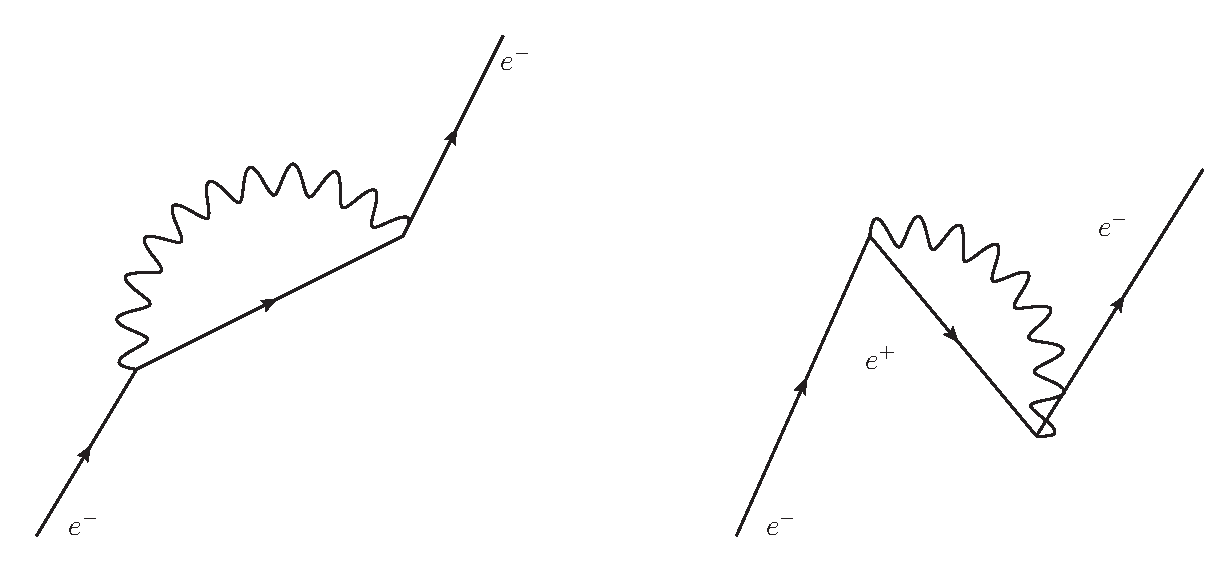
\includegraphics[width=0.8\linewidth]{fs-interpretation/fs-interpretation.eps}
   \caption{scattering process; horizontal time-axis; in the second diagram a electron positron pair is produced}%
   \label{fig:}
\end{figure}

In a relativistic systems we need to remember following points
\begin{itemize}
   \item anti-particles
   \item particle numbers are not conserved
\end{itemize}

\section{Electrodynamics (spin $1$)}
Maxwell equations are
\begin{align}
   \pmb{E} &= -\vec{\nabla} \phi - \frac{\dd}{\dd{t}}{\pmb{A}} \\
   \pmb{B} &= \vec{\nabla} \times \pmb{A}\\
   \vec{\nabla} \times \pmb{E} &= -\frac{\dd}{\dd{t}}{\pmb{B}} \\
   \div \pmb{B} &= 0
\end{align}

Field strength tensor and four-potential
\begin{align}
   F_{\mu\nu} &= \partial_\mu A_\nu - \partial_\nu A_\mu \\
   A^\mu(x) &= (\phi, \pmb{A})
\end{align}
The fields can be calculated from it
\begin{align}
   E^i &= F^{0i} = \partial^i A^0 - \partial ^0 A^i \\
   B_i &= -\epsilon_{ijk} \partial^i A^k = -\epsilon_{0ijk}F^{jk}
\end{align}

Often it is useful to use the dual tensor
\begin{align}
   \tilde{F}_{\mu\nu} &= \epsilon_{\mu\nu\sigma\tau} F^{\sigma \tau} \\
   \partial^{\mu} \tilde{F}_{\mu\nu} &= 0
\end{align}
is the second set of maxwell equations.

The other set of two equations is 
\begin{align}
   \partial_\nu F^{\mu\nu} = 4\pi j^\mu
\end{align}

$\pmb{E}, \pmb{B}$ are observable, $\pmb{A}$ is not. $A^\mu$ is not uniquely fixed by $\pmb{E}$ and $\pmb{B}$. It has the following gauge symmetry
\begin{align}
   \tilde{A}_{\mu} = A_\mu + \partial_\mu \Lambda(\pmb{x}, t)
\end{align}

Use this transformation to get
\begin{align}
   \partial_\mu A^\mu = 0
\end{align}

Plugging it back then we have the relativistic wave equation
\begin{align}
   \partial_\mu \partial^\mu A^\nu = 0
\end{align}
it essentially is Klein-Gordon equation with mass $m=0$

$A^\mu$ is a vector with spin $1$
\begin{align*}
   (j_+, j_-) = \left( \frac{1}{2}, \frac{1}{2} \right)
\end{align*}
It implied it has two transverse degrees of freedom. It has spin $1$ properties: $+1$, $0$, $-1$, in which $0$ mode does not exist.

\section{Description of Fermions}
Original motivation for Dirac. He wants a linear equation in $E$ or $\frac{\partial}{\partial t}$
\begin{align*}
   p^\mu \mapsto i\partial^\mu
\end{align*}

Take the ansatz
\begin{align*}
   i\hbar \frac{\partial}{\partial t}\psi &= H \psi \\
   &= (\vec{\alpha}\cdot \pmb{p} + \beta m ) \psi
\end{align*}
but $\pmb{\alpha}$ and $\beta$ unknown. It still has to obey the relativistic energy relation
\begin{align*}
   A &= \left( \alpha_ip_i + \beta m \right) \left( \alpha_ip_i + \beta m \right) \\
     &\stackrel{!}{=} \pmb{p}^2 + m^2 \\
     &= \alpha_i \alpha_j p_i p_j + \beta^2m^2 + \alpha_i \beta p_i m + \beta \alpha_j p_j m
\end{align*}

From this we demand
\begin{align}
   \beta^2 = 1 \\
   \alpha_i^2 = 1 \\
   \alpha_i \alpha_j + \alpha_j \alpha_i = 0 \\
   \alpha_i \beta + \beta \alpha_i = 0
\end{align}
So $\alpha$ and $\beta$ are not just numbers, but (can be proven to be) hermitian traceless matrices with eigenvalue $\pm 1$.  In addition, it only exits in even dimensions.
Since $\alpha_i$ and $\beta$ are $4\times4$ matrices. $\psi$ has to be a 4-component spinor.

For parity conservation need $(\frac{1}{2}, 0) \bigoplus (0, \frac{1}{2})$
Thus 
\begin{align*}
   \begin{pmatrix} \begin{pmatrix} & \\ & \end{pmatrix}_{2\times2} & \\ & \begin{pmatrix} & \\ &  \end{pmatrix}_{2\times2}   \end{pmatrix}
\end{align*}

There are different sets of $\alpha_i, \beta$ which satisfy the conditions. They are called representations.

Dirac-Pauli representation
\begin{align}
   \alpha_i &= \begin{pmatrix} 0 & \sigma^i \\ \sigma^i &  0 \end{pmatrix} \\
   \beta &= \begin{pmatrix} \id_2 & 0 \\ 0 & -\id_2\end{pmatrix}
\end{align}
with $\sigma^i$ the Pauli matrices.

Weyl (chiral) representation
\begin{align}
   \alpha^i &= \begin{pmatrix} -\sigma^i & 0 \\ 0 & \sigma^i \end{pmatrix}  \\
   \beta &= \begin{pmatrix} 0 & \id_2 \\ \id_2 & 0 \end{pmatrix}
\end{align}
they are mainly used in high energy physics (E $\gg m$).

\subsection{Gamma Matrices}
We now define 4 gamma matrices $\gamma^\mu$, $\mu=0,1,2,3$
\begin{align}
   \gamma^\mu = \left(\beta, \beta \pmb{\alpha} \right)
\end{align}
Note that having an index does not make it Lorentz vector.

The Clifford algebra is defined as following
\begin{align}
   \left\{ \gamma^\mu, \gamma^\nu \right\} = \gamma^\mu \gamma^\nu + \gamma^\nu \gamma^\mu = 2 g^{\mu\nu}
\end{align}

In Dirac-Pauli representation
\begin{align}
   \gamma^0 &= \begin{pmatrix} \id & 0 \\ 0 & -\id \end{pmatrix} \\
   \gamma^i &= \begin{pmatrix} 0 & \sigma^i \\ -\sigma^i & 0 \end{pmatrix} \\
   \gamma^5 &= i \gamma^0 \gamma^1 \gamma^2 \gamma^3 = \begin{pmatrix} 0 & \id \\ \id & 0\end{pmatrix}
\end{align}

In Weyl representation 
\begin{align*}
   \gamma^0 \leftrightarrow \gamma^5
\end{align*}

Rewriting the Dirac equation using $\gamma$s
\begin{align}
   i \partial_t \psi &= \left( \pmb{\alpha} \cdot \pmb{p} + \beta m  \right) \psi \notag\\
   i \partial_t \psi &= -i \pmb{\alpha} \cdot \vec{\nabla} \psi + m \beta \psi \notag\\
   i \beta \partial_t \psi &= -i \beta \pmb{\alpha} \cdot \vec{\nabla} \psi + m \psi \notag\\
   \left(i\gamma^\mu \partial_\mu - m \right) \psi &= 0
\end{align}
Conventionally we use $\phi$ for spin $0$ particle and $A_\mu$ for spin $1$.

It is convenient to also have an equation for $\psi^\dagger$. First one can show $\gamma^{\dagger\mu} = \gamma^0 \gamma^\mu \gamma^0$.
\begin{itemize}
   \item $\mu = 0$: $\gamma^0 = \beta$ and $\gamma^{\dagger\, 0} = \gamma^0 \gamma^0 \gamma^0$ $\Rightarrow \beta^2 = \id_4$
   \item $\gamma^{\dagger\mu} = (\beta \alpha^k)^\dagger = (\alpha^k)^\dagger \beta^\dagger = \alpha^k \beta = \beta^2 \alpha^k \beta = \beta \gamma^k \beta = \gamma^0 \gamma^k \gamma^0$
\end{itemize}

\begin{align}
   i \gamma^0 \partial_0 \psi + i \gamma^k \partial_k \partial - m \psi = 0 \notag\\
   -i \partial_0 \psi^\dagger (\gamma^0)^\dagger - i(\partial_k \psi^\dagger) \gamma^{\dagger\; k} - m \psi^\dagger = 0 \notag \\
   -i \partial_0 \psi^\dagger \gamma^0 - i(\partial_k \psi^\dagger) \gamma^0 \gamma^k \gamma^0 - m \psi^\dagger = 0 \notag \\
   \shortintertext{define $\bar{\psi} = \psi^\dagger \gamma^0$}
   -i \partial_0 \bar{\psi} \gamma^0 - i \partial_\mu \bar{\psi} \gamma^\mu - m \bar{\psi} = 0 \notag \\
   i(\partial_\mu \bar{\psi}) \gamma^\mu + m \bar{\psi} = 0
\end{align}

\subsection{Free Particle Solution to Dirac Equation}
\begin{align*}
   \left( i \gamma^\mu \partial_\mu - m \right) \psi &= 0 \\
   \shortintertext{multiplying $\gamma^\nu \partial_\nu$ from left}
   i\gamma^\mu \gamma^\nu \partial_\mu \partial_\nu \psi - m \gamma^\nu \partial_\nu \psi &= 0 \\
   i \gamma^\mu \gamma^\nu \partial_\mu \partial_\nu \psi + i m^2 \psi &= 0 \\
\end{align*}

\begin{align*}
   \gamma^\mu \gamma^\nu  &= \frac{1}{2} \left( \gamma^\mu \gamma^\nu + \gamma^\nu \gamma^\mu  \right) \\
                          &= \frac{1}{2} \left( \gamma^\mu \gamma^\nu - \gamma^\nu \gamma^\mu + 2g^{\mu\nu} \right) \\
                          &= \frac{1}{2} \left[ \gamma^\mu , \gamma^\nu \right] + g^{\mu\nu}
\end{align*}
The commutator is anti-symmetric and multiplying to symmetric tensor (derivatives) the term must vanish.

Each component of spinor satisfies the Klein-Gordon equation.
\begin{align}
   (\partial_\mu \partial^\mu + m^2) \psi_i = 0
\end{align}

Thus we can write the solution as plane-wave
\begin{align}
   \psi = u(\pmb{p}) \euler^{-ipx}
\end{align}
$u(\pmb{p})$ is also a 4-component object but as function $\pmb{p}$ not $\pmb{x}$

Insert back into Dirac equation, then we have Dirac equation in momentum space
\begin{align}
   \left( \gamma^\mu p_\mu - m \right) u(\pmb{p}) = 0
\end{align}

Solution by considering Dirac-Pauli representation
\begin{align*}
   \left( \slashed{p} - m \right) u(\pmb{p}) = \begin{pmatrix} (E-m) \id & - \pmb{p} \cdot \pmb{\sigma} \\ \pmb{p} \cdot \pmb{\sigma} & -(E+m) \id \end{pmatrix} 
   \begin{pmatrix} u_A \\ u_B\end{pmatrix}
\end{align*}

$\pmb{p} = 0$ then $E = \pm m$

\begin{itemize}
   \item $E = +m$ Two solutions 
      \begin{align*}
         u_B = \begin{pmatrix} 1 \\ 0 \end{pmatrix} , \begin{pmatrix} 0 \\ 1\end{pmatrix}
      \end{align*}

   \item $E=-m$
      \begin{align*}
         u_A = \begin{pmatrix} 1 \\ 0\end{pmatrix}, \begin{pmatrix} 0 \\ 1\end{pmatrix}
      \end{align*}
\end{itemize}

$\pmb{p} = 0$
\begin{align}
   \pmb{\sigma} \cdot \pmb{p} u_B &= (E-m) u_A \\
   \pmb{\sigma} \cdot \pmb{p} u_A &= (E+m) u_B
\end{align}

\begin{itemize}
   \item $E>0$ 
      \begin{align*}
         \chi^{(1)} &= \begin{pmatrix} 1 \\ 0\end{pmatrix} \\
         \chi^{(2)} &= \begin{pmatrix} 0 \\ 1\end{pmatrix}
      \end{align*}
\end{itemize}

Ansatz $u_A^{(s)} = \chi^{(s)}$
\begin{align}
   u_B^{(s)} = \frac{\pmb{\sigma}\cdot\pmb{p}}{E + m} &\quad u_A^{(s)} = \frac{\pmb{\sigma}\cdot\pmb{p}}{E + m} \chi^{(s)} \notag\\
   u(\pmb{p}) &= N \begin{pmatrix} \chi^{(s)} \\ \frac{\pmb{\sigma}\cdot\pmb{p}}{E + m} \chi^{(s)}\end{pmatrix}
\end{align}

$E < 0$ and $u_B^{(s)} = \chi^{(s)}$
\begin{align}
   u(\pmb{p}) = N \begin{pmatrix} -\frac{\pmb{\sigma}\cdot\pmb{p}}{E + m} \chi^{(s)} \\ \chi^{(s)}\end{pmatrix}
\end{align}

One can show $u^{\dagger (r)} u^{(s)} = N^2 \delta^{rs}$

Two fold degeneracy in each case. $ \begin{pmatrix} 1 \\ 0\end{pmatrix}$ and $ \begin{pmatrix} 0 \\ 1\end{pmatrix} $ for $E > 0$ and $E < 0$. There must be another observable which commutes with $H$ and $\pmb{p}$.
\begin{align*}
   H = \gamma^i p_i + \gamma^0 m
\end{align*}
\begin{align}
   \pmb{S} \cdot \hat{P} = \frac{1}{2} \begin{pmatrix} \pmb{\sigma}\cdot\pmb{p} & 0 \\ 0 & \pmb{\sigma}\cdot \hat{p}\end{pmatrix}
\end{align}

Helicity
\begin{align}
   \frac{1}{2} \pmb{\sigma} \cdot {\hat{p}} &= \frac{1}{2} \begin{pmatrix} \hat{p}_z & \hat{p}_x + i\hat{p}_y \\ \hat{p}_x -i \hat{p}_y & -\hat{p}_z\end{pmatrix} \\
   \det(\pmb{\sigma} \cdot \hat{p}) &= - \hat{p}^2 = - 1
\end{align}
  
Determinant is the product of two eigenvalues, then
\begin{align*}
   \lambda_1 + \lambda_2 &= 0 \\
   \lambda_1 \cdot \lambda_2 &= 1 \\
   \lambda_{1,2} &= \pm 1
\end{align*}

Antiparticle solution $u^{(3,4)}(-\pmb{p}) e^{-i(-p)x} = v^{(2,1)}$
\begin{align}
   \left( \slashed{p} + m \right)v(\pmb{p}) = 0
\end{align}

Normalization is
\begin{align}
   \int \rho \dd{V} = 2E \\
   N = \sqrt{E+m}
\end{align}

Completeness relation (spin sums)
\begin{align}
   \sum u^{(s)}(p) \bar{u}^{(s)}(p ) = \left( \slashed{p} + m \right) \\
   \sum v^{(s)}(p) \bar{v}^{(s)}(p ) = \left( \slashed{p} - m \right)
\end{align}

Define a projector projecting out positive and negative energy states
\begin{align}
   \Lambda_{\pm} = \frac{\pm \slashed{p} + m}{2m}
\end{align}

In Chiral (Weyl) representation
\begin{align}
   \left( \slashed{p} - m \right) u(\pmb{p}) = \begin{pmatrix} m & p \cdot \sigma \\ \vecp \cdot \bar{\sigma} & -m \end{pmatrix} \begin{pmatrix} u_L \\ u_R\end{pmatrix}
\end{align}
$\bar{\sigma} = (\sigma^0 , -\pmb{\sigma})$ and $\sigma^0 = \id_2$

Weyl equation
\begin{align}
   \begin{split}
    -m u_L + p\cdot \sigma u_R = 0 \\
   p \cdot \bar{\sigma} u_L - m u_R = 0
   \end{split}
\end{align}
if $m=0$, the equations decouple from each other.

%%%%%%%%%%%%%%%%%%%%%%%%%%%%%%%%%%%%%%%%%%%%%%%%%%%%%%%%%%%%%%%
% Lecture on 21.10
%%%%%%%%%%%%%%%%%%%%%%%%%%%%%%%%%%%%%%%%%%%%%%%%%%%%%%%%%%%%%%%

We want to construct Lagrangians involving the fields $\psi$, $A_\mu$ and $\psi$. The reason we choose Lagrangians as opposed to Hamiltonians, is that Hamiltonian $H$ is associated with energy of system, which is not Lorentz (or relativistic) invariant. But Lagrangian density is $S = \int \dd{t} = \int \dd[4]{x} \lag$. In natural unit, the action is dimensionless. One can in addition prove $\dd[4]{x}$ is Lorentz invariant.  The fact that $\lag$ is Lorentz invariant, means that $\lag$ need to have at least $2$ spin-$\frac{1}{2}$ fields $\psi$ or $\bar{\psi}$, to make a spin-$0$.

We are interested in the objects like
\begin{align*}
   \bar{\psi}(\gamma^\mu) \psi
\end{align*}

Representation of the Lorentz group can be split into $ \left( \frac{1}{2}, 0 \right)$ and $ \left( 0, \frac{1}{2} \right)$. In Weyl or chiral representation, $\psi_L$ has $ \left( \frac{1}{2}, 0 \right)$ and $\psi_R$ $ \left( 0, \frac{1}{2} \right)$.

Here we are taking a different approach from the paper \cite{Dreiner_2010}. First define
\begin{align}
   \sigma^{\mu\nu} = \frac{i}{2} \left[ \gamma^\mu, \gamma^\nu \right]
\end{align}

We want to find out the transformation of $\psi = u(\pmb{p})e^{-ip\cdot x}$. Note that the second factor is written in covariant form, i.e.~Lorentz invairant. Consider the Dirac equation in two different frames $x' = \Lambda x$
\begin{align}
   i \gamma^\mu \frac{\partial \psi(x)}{\partial x^\mu} - m \psi(x) = 0 \label{math:dirac}\\
   i \gamma^\mu \frac{\partial \psi'(x')}{\partial x'^\mu} - m \psi'(x') = 0 \label{math:diracP}
\end{align}

We make the ansatz that the spinor transforms with $S$ 
\begin{align}
   \psi'(x') = S\psi(x) \label{math:psiS}
\end{align}
$S$ must be independent of $x$. Plug \ref{math:psiS} into \ref{math:diracP} 
\begin{align*}
   i \gamma^\mu \frac{\partial}{\partial x'^\mu} \left[ S \psi(x) \right] - m S \psi(x) &= 0 \\
   i S^{-1} \gamma^\mu S \frac{\partial \psi (x)}{\partial x^\nu} \underbrace{\frac{\partial x^\nu}{\partial x'^\mu}}_{=\Lambda^{-1}} - m\psi(x)  &= 0
\end{align*}

This equation must be the same as \ref{math:dirac}, then we get
\begin{align}
   S^{-1} \gamma^\mu S \left[ \Lambda^{-1} \right]^\nu_{\; \mu} &= \gamma^\nu \notag\\
   S^{-1} \gamma^\mu S &= \Lambda^\mu_{\; \nu} \gamma^\nu
\end{align}

$S_{\mu\nu}$ is anti-symmetric in $\mu$ and $\nu$
\begin{align}
   S_i &= \frac{1}{2} \epsilon_{ijk} S^{jk} \\
   K_i &= S^{0i} \\
   \psi'_\alpha(x') &= \left[\exp(-\frac{i}{2} \Theta^{\mu\nu} S_{\mu\nu})\right]^\beta_\alpha \psi_\beta \\
   \omega_i &= \frac{1}{2} \epsilon_{ijk} \theta_{ijk}
\end{align}

Lorentz transformation containing rotations and boosts, but infinitesimal version (infinitesimally different from $\id$)
\begin{align}
   \Lambda^\nu_{\; \mu} = \delta^\nu_{\;\mu} + \epsilon^\nu_{\;\mu}
\end{align}

We will show in the exercise the expression of transformation under boosts and rotations
\begin{align}
   S_L &= \id_4 - \frac{i}{4} \sigma_{\mu\nu} \epsilon^{\mu\nu} \\
   S_L^{-1} &= \id_4 + \frac{i}{4} \sigma_{\mu\nu} \epsilon^{\mu\nu}
\end{align}

It satisfies $S^{-1} \gamma^\mu S = \Lambda^{\mu}_{\;\nu} \gamma^\nu = \gamma^\nu + \epsilon^\mu_{\;\nu} \gamma^\nu$
\begin{align*}
   \left(\id_4 + \frac{i}{4} \sigma_{\mu\nu} \epsilon^{\mu\nu} \right) \gamma^\mu \left(\id_4 - \frac{i}{4} \sigma_{\mu\nu} \epsilon^{\mu\nu}\right)
   &= \gamma^\mu + \frac{i}{4} \left[ \sigma_{\alpha\beta} \gamma^\mu - \gamma^\mu \sigma_{\alpha\beta} \right]\epsilon^{\alpha \beta} 
   \shortintertext{somehow}
   &= \gamma^\mu + \epsilon^\mu_{\; \nu} \gamma^\nu
\end{align*}

Parity transformation cannot be written in infinitesimal form. Thus it is often called (one of) discrete transformation.
\begin{align}
\Lambda_{\text{P}} = \diag(+1,-1,-1,-1)
\end{align}
Parity symmetry is naturally violated. Especially in weak interaction, since neutrinos are left-handed $\nu_L$.
\begin{align}
   S^{-1}_\text{P} \gamma^\mu S_\text{P} = \Lambda^\mu_{\text{P}\, \nu} \gamma^\nu
\end{align}

\begin{itemize}
   \item For $\mu = 0$ 
      \begin{align*}
S^{-1}_\text{P} \gamma^0 S_\text{P} = \gamma^0
      \end{align*}
   \item For $\mu=i$
      \begin{align*}
S^{-1}_\text{P} \gamma^i S_\text{P} = -\gamma^i
      \end{align*}
\end{itemize}

It is easy to show $S_\text{P} = \gamma^0$ satisfies the equations. Then the spinor transform under parity like
\begin{align}
   \psi'(t, -\pmb{x}) = \gamma^0 \psi(t,\pmb{x})
\end{align}

In Dirac-Pauli representation $\gamma^0 = \begin{pmatrix} \id_2 & 0 \\ 0 & \id_2 \end{pmatrix}$
\begin{align*}
   \psi = \begin{pmatrix} \psi_1 \\ \psi_2 \\ \psi_3 \\ \psi_4 \end{pmatrix} \quad
   \psi' = \begin{pmatrix} \psi_1 \\ \psi_2 \\ -\psi_3 \\ -\psi_4 \end{pmatrix} 
\end{align*}

In chiral representation $\gamma^0 = \begin{pmatrix} 0 & \id_2 \\ \id_2 & 0 \end{pmatrix}$ and 
\begin{align*}
\psi = \begin{pmatrix} \psi_L \\ \psi_R\end{pmatrix} \quad
\psi' = \begin{pmatrix} \psi_R \\ \psi_L \end{pmatrix}
\end{align*}

Recall $\bar{\psi} = \psi^\dagger \gamma^0$. 
\begin{align*}
   \bar{\psi}' &= \psi'^\dagger \gamma^0 = \psi^\dagger S^\dagger \gamma^0 \\
   \shortintertext{it can easily be shown using the explicit expresseion of $S_L$ and $S_L$. Parity transformation is $\gamma^0$.}
               &= \psi^\dagger \gamma^0 S^{-1} \\
               &= \bar{\psi} S^{-1}
\end{align*}

There are $16$ different bilinear $\bar{\psi} A \psi$
\begin{itemize}
   \item $A = \id_4$
      \begin{align*}
      \bar{\psi}' \psi' = (\bar{\psi} S^{-1}) (S \psi) = \bar{\psi} \psi
      \end{align*}
   \item $A = \gamma^\mu$
      \begin{align*}
          \bar{\psi}' \gamma^\mu \psi' = \bar{\psi} S^{-1} \gamma^\mu S \psi = \Lambda^\mu_{\;\nu} \left( \bar{\psi} \gamma^\nu \psi \right)
      \end{align*}
      It transforms exactly like a Lorentz vector. Especially under parity
      \begin{align*}
         \bar{\psi}' \gamma^\mu \psi' = \begin{cases}
            \bar{\psi}' \gamma^0 \psi'  & \mu = 0 \\
            -\bar{\psi}' \gamma^i \psi'   & \mu = 1,2,3
         \end{cases}
      \end{align*}
   \item $A = \gamma^5$
      \begin{align*}
         \bar{\psi}' \gamma^5 \psi' &= \bar{\psi} S_L^{-1} \gamma^5 S_L \psi 
          \shortintertext{$ \left\{ \gamma^\mu, \gamma^5 \right\} = 0$ and  $\sigma_{\mu\nu}$ contains two $\gamma$s}
                                    &= \bar{\psi} \gamma^5 \psi 
      \end{align*}
      It is a scalar under boosts and rotations.
      Under parity it is pseudoscalar, like pions.
      \begin{align*}
         \gamma^5 S_\text{P} = \gamma^5 \gamma^0 = - S_\text{P} \gamma^5
         \shortintertext{thus}
            \bar{\psi}' \gamma^5 \psi' = - \bar{\psi}' \gamma^5 \psi'
      \end{align*}

      For experiments, look it up in Introduction to HEP, Perkins
\end{itemize}

Chiral spinors (in chiral representation)
\begin{align}
   P_R &= \frac{1}{2} \left( \id_4 + \gamma^5 \right) = \begin{pmatrix} 0&0\\0&\id_2\end{pmatrix} \\
   P_L &= \frac{1}{2} \left( \id_4 - \gamma^5 \right) = \begin{pmatrix} \id_2&0\\0&0\end{pmatrix}
\end{align}

If $\psi$ written like $\psi = \begin{pmatrix} \chi_L \\ \chi_R \end{pmatrix}$, it is in chiral representation
\begin{align*}
   P_L \psi &= \begin{pmatrix} \chi_L \\ 0\end{pmatrix} = \psi_L \\
   P_R \psi &= \begin{pmatrix} 0 \\ \chi_R \end{pmatrix} = \psi_R
\end{align*}

They are projectors
\begin{align*}
   P_R^2 &= \frac{1}{4} (\id_4 + \gamma^5) (\id_4 + \gamma^5) = \frac{1}{4} (\id_4 + 2 \gamma^5 + (\gamma^5)^2) = P_R \\
   P_L^2 &= P_L
\end{align*}

They also project onto complete space meaning $P_L + P_R = \id_4$.

Left-handed particles have spin and momentum in the opposite direction and right-handed in the same direction. In Dirac-Pauli representation in high energy limit
\begin{align*}
   \gamma^5 u^{(5)} \approx \begin{pmatrix} \pmb{\sigma} \cdot \hat{p} & 0 \\ 0 & \pmb{\sigma} \cdot \hat{p}\end{pmatrix}
\end{align*}

To show this take the free particle solution ($E>0$)
\begin{align*}
   u^{(s)} &= N \begin{pmatrix} \chi^{(s)} \\ \frac{\pmb{\sigma \cdot \pmb{p}}}{E+m} \chi^{(s)}\end{pmatrix} \\
   \gamma^5 u^{(s)} &= N  \begin{pmatrix}  \frac{\pmb{\sigma \cdot \pmb{p}}}{E+m} \chi^{(s)} \\ \chi^{(s)}  \end{pmatrix} \approx N \begin{pmatrix} \pmb{\sigma} \cdot \hat{p} \chi^{(s)} \\ \chi^{(s)} \end{pmatrix} \\
   \shortintertext{In general $(\pmb{\sigma \cdot \pmb{a}})^2 = \pmb{a}^2 \id$} 
   &=  N \pmb{\sigma} \cdot \hat{p} \begin{pmatrix} \chi^{(s)} \\ \pmb{\sigma} \cdot \hat{p} \chi^{(s)} \end{pmatrix}  = \underbrace{\pmb{\sigma} \cdot \hat{p}}_{\text{helicity operator}} u^{(s)} \\
\end{align*}

At high energy limit ($E \gg m$), $\gamma^5$ helicity operator, but not at low energy. Chirality $\psi_{L,R}$ is always a good quantum number.

%%%%%%%%%%%%%%%%%%%%%%%%%%%%%%%%%%%%%%%%%%%%%%%%%%%%%%%%%%%%%%%%%%%%%%
% Lecture on 22.10 
%%%%%%%%%%%%%%%%%%%%%%%%%%%%%%%%%%%%%%%%%%%%%%%%%%%%%%%%%%%%%%%%%%%%%

\paragraph{Angular momentum}
Must be another observable which commutes with $H$ and $P$ (u = u(\pmb{p}))
\begin{align}
   \pmb{\Sigma} \cdot \hat{p} &= \begin{pmatrix} \pmb{\sigma} \cdot \hat{p} & 0 \\ 0 &\pmb{\sigma} \cdot \hat{p} \end{pmatrix} \\
   H &= \alpha \cdot P + \beta m \\
   \left[ H, \pmb{\Sigma} \cdot \hat{p} \right] &= 0
\end{align}

Angular momentum operator is defined as 
\begin{align}
   \pmb{L} = \pmb{r} \times \pmb{P} \\
\end{align}

Use the relation $\left[ \hat{x}_i, \hat{P}_j \right] = i \delta_{ij}$ and check the commutation
\begin{align*}
   \left[ H, L_1 \right] &= \left[ \pmb{\alpha} \cdot \pmb{P}, x_2 P_3 - x_3 P_2 \right] \\
                         &= \left[ \alpha_1 P_1 + \alpha_2 P_2 + \alpha_3 P_3, x_2 P_3  - x_3 P_2 \right] \\
                         &= \alpha_2 \left[ P_2, x_2 \right] P_3 - \alpha_3 \left[ P_3, x_3 \right] P_2  \\
                         &= -i \left( \alpha_2 P_3 - \alpha_3 P_2 \right)\\
                         &= -i (\alpha \times P)_1
\end{align*}
Thus $ \left[ H, \pmb{L} \right] = -i (\pmb{\alpha} \times P) \neq 0$. In other word, $L$ not conserved.

But we observe
\begin{align}
   \pmb{\Sigma} &= \begin{pmatrix} \pmb{\sigma} & 0 \\ 0 & \pmb{\sigma}\end{pmatrix} \\
   \left[ H, \pmb{\Sigma} \right] &= 2i(\pmb{\alpha} \times P)
\end{align}
Thus define total angular momentum, second term describe the intrinsic angular momentum of particles
\begin{align}
   \pmb{J} = \pmb{L} + \frac{1}{2} \pmb{\Sigma}
\end{align}
and $J$ is conserved.

\paragraph{Charge conjugation}
Equation describing fermions couple to electromagnetic current
\begin{align}
   \left[ \gamma^\mu \left( i \partial_\mu + e A_\mu \right) - m \right] \psi = 0 \label{math:diracEM}
\end{align}
with $e$ the electric charge of electron and $A_\mu(x)$ vector potential in electromagnetism.
 
For positron the charge is the opposite
\begin{align}
   \left[ \gamma^\mu \left( i \partial_\mu - e A_\mu \right) - m \right] \psi^\text{C} = 0 \label{math:diracEMP}
\end{align}
$\psi^{\text{C}}$ is the charge conjugate of  $\psi$. We want to know the relation between $\psi \leftrightarrow \psi^{\text{C}}$. Take complex conjugate of equation \ref{math:diracEM}
\begin{align}
   \left[ -(\gamma^{\mu})^{*} \left( i \partial_\mu - eA_\mu \right) - m \right] \psi^* &= 0 \label{math:diracEMCC}
   \shortintertext{We postulate a matrix $C$ so that $\psi^\text{C} = C\gamma^0 \psi^*$ and multiply equation \ref{math:diracEMCC} by $C \gamma^0$ from left. }
   C \gamma^0 \left[ -\left(\gamma^{\mu}\right)^* \left( i \partial_\mu - eA_\mu \right) - m \right] \psi^* &= 0 \notag \\
   \shortintertext{It must be the same as equation \ref{math:diracEMP}. Thus}
   - (C \gamma^0) (\gamma^{\mu})^{*} &= \gamma^\mu C \gamma^0 \notag \\
   - C (\gamma^{\mu})^{\text{T}} &= \gamma^\mu C \notag \\
   C \gamma^{\mu T} C^{-1} &= - \gamma^\mu \notag \\
   C &= i \gamma^0 \gamma^2
\end{align}

Then we find
\begin{align}
   \psi^{\text{C}} = C \gamma^0 \psi^* = C \bar{\psi}^\text{T}
\end{align}

It would be interesting to compare $P_L (\psi^\text{C})$ and $(P_L \psi)^\text{C}$

\paragraph{Continuity equation for $\psi$}
\begin{align}
   \rho = \psi^\dagger \psi = \bar{\psi} \gamma^0 \psi
\end{align}
Multiply $\bar{\psi}$ from left to dirac equation and $\psi$ from right to conjugated Dirac equation
\begin{align*}
   \bar{\psi} \left( i \gamma^\mu \partial_\mu - m \right) \psi = 0, &\qquad i (\partial_\mu \bar{\psi}) \gamma^\mu \psi + m \bar{\psi} \psi = 0\\
   \bar\psi \gamma^\mu (\partial_\mu \psi) + (\partial_\mu \bar\psi) \gamma^\mu \psi &= 0 \\
   \partial_\mu ( \bar{\psi} \gamma^\mu \psi) &= 0 \\
   \partial_\mu j^\mu &= 0
\end{align*}

\section{Classical Field Theory} 
\paragraph{Reminder} 
\begin{align*}
   \shortintertext{Lagrangian and action}
   L = L (q_i, \dot{q}_i, t) &\qquad   S = \int \dd{t} L \\
   \shortintertext{Variantion principle}
   \delta S &= 0 \\
   \shortintertext{is equivalent to Euler-Lagrange equations}
   \frac{\dd}{\dd{t}} \frac{\partial L}{ \partial \dot{q}_i}& =\frac{\partial L}{\partial q_i}
\end{align*} 

Going to field theory, we transform $q(t) \rightarrow \phi(x)$ and $L \rightarrow \lag$
\begin{align*}
   \lag &= \lag \left(\phi, \frac{\partial \phi}{\partial x^\mu}, x_\mu \right) \\
   S &= \int \dd[4]{x} \lag(\phi, \frac{\partial \phi}{\partial x^\mu}, x_\mu) 
\end{align*}

Using the variation principle
\begin{align*}
   \delta S &= \sum_i \frac{\dd{S}}{\dd{\alpha_i}} \delta \alpha_i \\
            &= \sum_i \int \dd[4]{x} \left\{ \frac{\partial \lag}{\partial \phi} \frac{\partial \phi}{\partial \alpha_i} \delta \alpha_i + \frac{\partial \lag}{\partial (\partial_\mu \phi)} \frac{\partial (\partial_\mu \phi)}{\partial \alpha_i} \delta \alpha_i \right\} \\
            &= \sum_i \int \dd[4]{x} \left\{ \frac{\partial \lag}{\partial \phi} \frac{\partial \phi}{\partial \alpha_i} - \left( \partial_\mu \frac{\partial \lag}{\partial (\partial_\mu \phi)} \frac{\partial \phi}{\partial \alpha_i} \right) \right\}\delta \alpha_i + \eval{\frac{\partial \lag}{\partial (\partial_\mu \phi)} \frac{\partial \phi}{\partial \alpha_i} \delta\alpha_i}_{x_0}^{x_1}
\end{align*}

Then we have our new Euler-Lagrange equations for continuous fields
\begin{align}
   \frac{\partial \lag}{\partial \phi} - \partial_\mu \frac{\partial \lag}{\partial(\partial_\mu \phi)} = 0
\end{align}

\paragraph{Conservation Laws and Noether Theorem}
Reminder: Under transformation $t \mapsto t' = t + \delta b$, system stays invariant if $\delta_T L = \frac{\dd}{\dd{t}}(\delta \Omega)$.

$\delta \Omega = 0$ if $L$ invariant

\begin{align*}
   \delta_T L = L(q, \dot{q}, t+\delta b) - L (q, \dot{q}, t) = \frac{\partial L}{\partial t} \delta b
\end{align*}

\begin{align*}
   \frac{\dd{L}}{\dd{t}} &= \frac{\partial L}{\partial t} + \frac{\partial L}{\partial q} \dot{q} + \frac{\partial L}{\partial \dot{q}} \ddot{q} \\
                         &= \frac{\partial L}{\partial t} + \frac{\dd}{\dd{t}} \left (\frac{\partial L}{\partial \dot{q}} \right) \dot{q} + \frac{\partial L}{\partial \dot{q}} \ddot{q} \\
                         &= \frac{\partial L}{\partial t} + \frac{\dd}{\dd{t}} \left[ \frac{\partial L}{\partial \dot{q}} \dot{q} \right] \\
\end{align*}

System invariant if
\begin{align}
   \frac{\partial L}{\partial t} = \frac{\dd}{\dd{t} } (\delta \Omega)
\end{align}
if $L$ not dependent explicitly on $t$, $\dd{L} / \dd{t} = 0$

If $\partial L / \partial t = 0$, the conserved quantity
\begin{align*}
   \frac{\dd}{\dd{t}} \left[ L - \frac{\partial L}{\partial \dot{q}} \dot{q} \right] &= 0 \\
   L - \frac{\partial L}{\partial \dot{q}} \dot{q} &= -H = L - \dot{q} p
\end{align*}
using legendre transformation and $\partial L / \partial \dot{q}$ the general momentum.

Analogously for fields
\begin{align*}
   \frac{\partial \lag}{\partial x^\mu} &= \left(\frac{\partial \lag}{\partial \phi} \right) \frac{\partial \phi}{\partial x^\mu} + \frac{\partial \lag}{ \partial (\partial_\rho \phi)} \partial_\rho (\partial_\mu \phi) \\
                                        &= \left(\partial_\rho \frac{\partial \lag}{\partial(\partial_\rho \phi)} \right) \partial_\mu \phi + \frac{\partial \lag}{ \partial (\partial_\rho \phi)} \partial_\rho \partial_\mu \phi \\
                     \partial_\mu \lag &= \partial_\rho \left[ \frac{\partial \lag}{\partial(\partial_\rho \phi)} \partial_\mu \phi \right]  \\
                                       &\Rightarrow \partial_\rho \left[ \lag \delta_{\mu}^{\rho} - \frac{\partial \lag}{\partial (\partial_\rho \phi)} \partial_\mu \phi \right] = 0
\end{align*}
this is energy momentum tensor $T_{\mu}^{\rho}$.

\paragraph{Examples}
Real scalar field, $\phi(x) \in \R$
\begin{align}
   \lag = \frac{1}{2} (\partial_\mu \phi) (\partial^\mu \phi) - \frac{1}{2} m^2 \phi^2
\end{align}
Since $L = T - V$, we interpret first term as kinetic and second as potential, which has minimum at $\phi=0$
Since action is dimensionless, $[\phi] = 1$. Take Euler-Lagrange 
\begin{align*}
   \frac{\partial \lag}{\partial \phi} = - m^2 \phi \\
   \frac{\partial \lag}{\partial (\partial_\mu \phi)} = \partial^\mu \phi \\
   \shortintertext{put together}
   \left( \partial_\mu \partial^\mu + m^2 \right)\phi = 0
\end{align*}
This is just Klein-Gordon equation. In Feynman rules we have the propagator and mass term as interaction

\paragraph{Example}Fermionic field
\begin{align}
   \lag = i \bar{\psi} \gamma_\mu \partial^\mu \psi - m \bar{\psi} \psi
\end{align}
$[\psi] = \frac{3}{2}$. $\bar\psi$ and $\psi$ are independent fields. Solve Euler-Lagrange we get familiar Dirac equation.
\begin{align}
   \frac{\partial \lag}{\partial \bar\psi}i \gamma_\mu \delta^\mu \psi - m \psi = 0
\end{align}

\paragraph{Example} Spin $1$ field $A_\mu(x)$
\begin{align}
   \lag = - \frac{1}{4} F_{\mu\nu} F^{\mu\nu} - j^\mu A_\mu \\
   F_{\mu\nu} = \partial_\mu A_\nu - \partial _\nu A_\mu
\end{align}

Equation of motion can be computed
\begin{align*}
   \frac{\partial \lag}{\partial (\partial_\rho A_\sigma)} &= \frac{1}{4} 4 \delta_{\rho \nu} \delta_{\mu \sigma} F^{\mu\nu} = - F^{\sigma \rho} \\
   \frac{\partial \lag}{\partial A_\sigma} &= - j^\sigma \\
   \shortintertext{then we have the maxwell equations}
   - \partial_\rho F^{\sigma \rho} + j^{\sigma} &= 0
   \shortintertext{use Lorenz gauge we can get}
   \partial_\mu \partial^\mu A^\sigma &= j^\sigma
\end{align*}
